\documentclass[
    xcolor={svgnames},
    hyperref={colorlinks,citecolor=OrangeRed,linkcolor=OrangeRed,urlcolor=DarkBlue}
    ]{beamer}
\setbeamerfont{caption}{size=\tiny}

\definecolor{LightPurple}{HTML}{bc83ff}

\usepackage{graphicx}
\graphicspath{{../images/}}

\usepackage{subcaption}
\usepackage{tabularx}
\usepackage{nameref}
\usepackage{amssymb,amsmath,amsthm}
\usepackage{adjustbox}

\usepackage{bookmark}

\newcommand{\linksection}[1]{\hyperlink{section:#1}{\nameref{section:#1}}}

\defbeamertemplate*{title page}{customized}[1][]
{
  \begin{center}
    \usebeamerfont{institute}\Huge\insertinstitute\par      
  \end{center}
  \centering
  \usebeamerfont{title}\LARGE\inserttitle\par
  \usebeamerfont{subtitle}\Large\insertsubtitle\par
  \bigskip
  \small\usebeamerfont{author}\insertauthor\par
  \usebeamerfont{date}\insertdate\par
}


\institute{Alma Mater Studiorum \\ University of Bologna}
\title{Artificial Intelligence \\ Machine Learning for Computer Vision}
\subtitle{Project work}
\author{Alessandro Dicosola [Matr. 935563]}
\date{}


\begin{document}
\begin{frame}
    \titlepage
\end{frame}

\begin{frame}{Task}
    SR is an \textcolor{red}{Ill-posed problem}: trying to create a mapping between LR to HR for \textcolor{blue}{reconstructing} SR images
    
    Keywords: super-sampling, super-resolution.
\end{frame}

\begin{frame}{Related works}
    \only<1>{
        \framesubtitle{SR through internal and external database\cite[Releated works]{LapSRN}}
        \small
        Exploit similarity between textures in images therefore create pairs of LR-HR patches for learning a low dimensional space were apply k-NN, non linear regressor, random forest, ... ,

        manifold embedding\cite[2004]{SRneighbporembedding}:
        \begin{columns}
            \begin{column}{0.5\textwidth}
                \begin{itemize}
                    \tiny
                    \item LR patches embedding is the concatenation of the first and second order derivative of the luminance at each pixel on the patch in the YIQ domain. 
                    \item HR patches embedding is the concatenation of all luminance at each pixel
                    \item Given a LR patch find the k-NN patches on the training set $$N_q$$
                    \item Compute the reconstruction weights minimizing the reconstruction error: $$argmin_W || x_t^q - \sum_{x_s^p \in N_q} w_{qp}x_s^p ||^2$$
                    \item Reconstruct the HR patch: $$y_t^q = \sum_{x_s^p \in N_q} w_{qp}y_s^p$$
                    \item Reconstruct the image overlapping the patches ( averaging on overlapped regions)
                \end{itemize}            
            \end{column}
            \begin{column}{0.5\textwidth}
                
                \begin{figure}
                    \centering
                    \begin{subfigure}[l]{0.55\textwidth}
                        \vspace*{-50px}
                        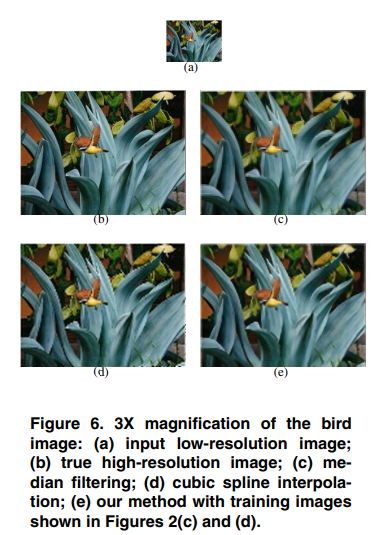
\includegraphics[height=0.30\textheight, keepaspectratio]{result-neighbour-embedding.png}
                    \end{subfigure}
                    \begin{subfigure}[l]{0.55\textwidth}
                        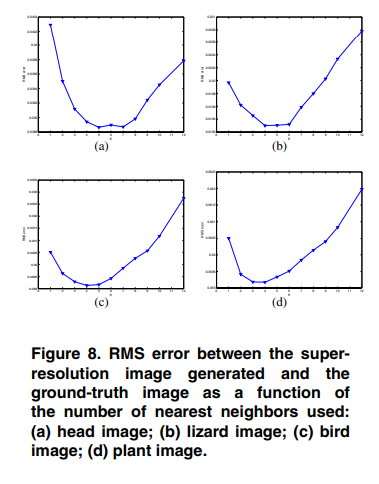
\includegraphics[height=0.30\textheight, keepaspectratio]{rms-neighbour-embedding.png}                    
                    \end{subfigure}
                \end{figure}
            \end{column}
        \end{columns}
    }
    % TODO: Create link to section
    \only<2>{
        \framesubtitle{CNN \cite[Releated works]{ASDN} \cite{SRsurvey}}
        \begin{itemize}
            \item SRCNN \cite{srcnn} : CNN using only three convolutions for extracting information, process them and reconstruct the SR image.
            \item VDSR : VGG-net that learns a residual instead of the direct mapping LR-HR in order to focus the training on high frequency information.
            \item SRDenseNet, RDN, \linksection{DBDN}\cite{DBDN}: Combine residual connection (locally and globally) with dense connection
            \item \linksection{RCAN}\cite{RCAN}, \linksection{CSFM}\cite{CSFM}: Use channel-wise and spatial attention for focusing the training on important features or region in order to ease the convergence and improve the results.
            \item \linksection{LapSRN}\cite{LapSRN}\cite{MSLapSRN} : multi scale network using a \textit{Laplacian Pyramid Framework} \linksection{LaplacianPyramid}\cite{laplacianpyramid}
            \item \linksection{MetaSR}\cite{MetaSR} : use a meta-upscaling module for learning LR-HR mapping using any scale.
        \end{itemize}
    }
\end{frame}

\begin{frame}{ASDN - Arbitrary-Scale Deep Network}
    \only<1>{
        \begin{itemize}
            \item Find an LR-HR mapping with \textcolor{blue}{any} scale (integer or real)
            \item Use Laplacian Frequency Representation for reconstructing SR image interpolating two nearest level in the LFR.
            \item The range scales was found to be optimal between 1 and 2 using 11 levels in the LFR.
            \item For scale greater than 2 the network is \textit{deployed recursively}.
        \end{itemize}
    }

    \only<2>{
        \framesubtitle{Laplacian Frequency Representation}
        \begin{figure}
            \centering
            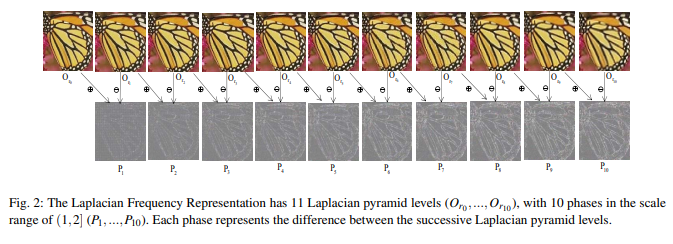
\includegraphics[height=0.3\textheight, keepaspectratio]{asdn-laplacian-pyramid.png}
        \end{figure}
        \begin{itemize}
            \item Learning any decimal scale is not possible: infinite decimal scales.
            \item Allow to have reduced dataset.
            \item Reconstruct the SR image interpolating the two nearest level in the LFR.
            \item Each level learn the HR representation at particular scale in the range.
            \item Compute the \textit{phase} as the difference between two consecutive levels in order to acquire \textbf{high frequency information}: $$ P_i = O_{r_{i-1}} - O_{r_i} $$
        \end{itemize}
    }

    \only<3>{
        \framesubtitle{Laplacian Frequency Representation}
        \begin{itemize}
            \item The scale for each level is:
            $$r_l = \frac{l}{L-1} + 1$$
            therefore the level can be indexed as
            $$l = (r_l - 1) * (L-1)$$
            $$i = \left\lceil (r - 1) * (L - 1) \right\rceil $$
            \item Define the weight, proportional to the distance between the scales, as:
            $$w_r = (L - 1)*(r_i - r)$$
            \item The SR image is reconstructed as:
            $$O_r = O_{r_i} + w_r \ast P_i $$
        \end{itemize}
    }
    \only<4>{
        \framesubtitle{Example}
        $$r = 1.27$$
        $$i = \left\lceil 10 * (1.27 - 1)\right\rceil = \left\lceil2.7\right\rceil = 3$$
        $$w_r = 10 * (1.3 - 1.27) = 0.3$$
        $$O_r = O_{r_3} + 0.3 \ast P_3$$
    }
    \only<5>{
        \framesubtitle{Study of Laplacian Frequency Representation}
        \begin{figure}
            \centering
            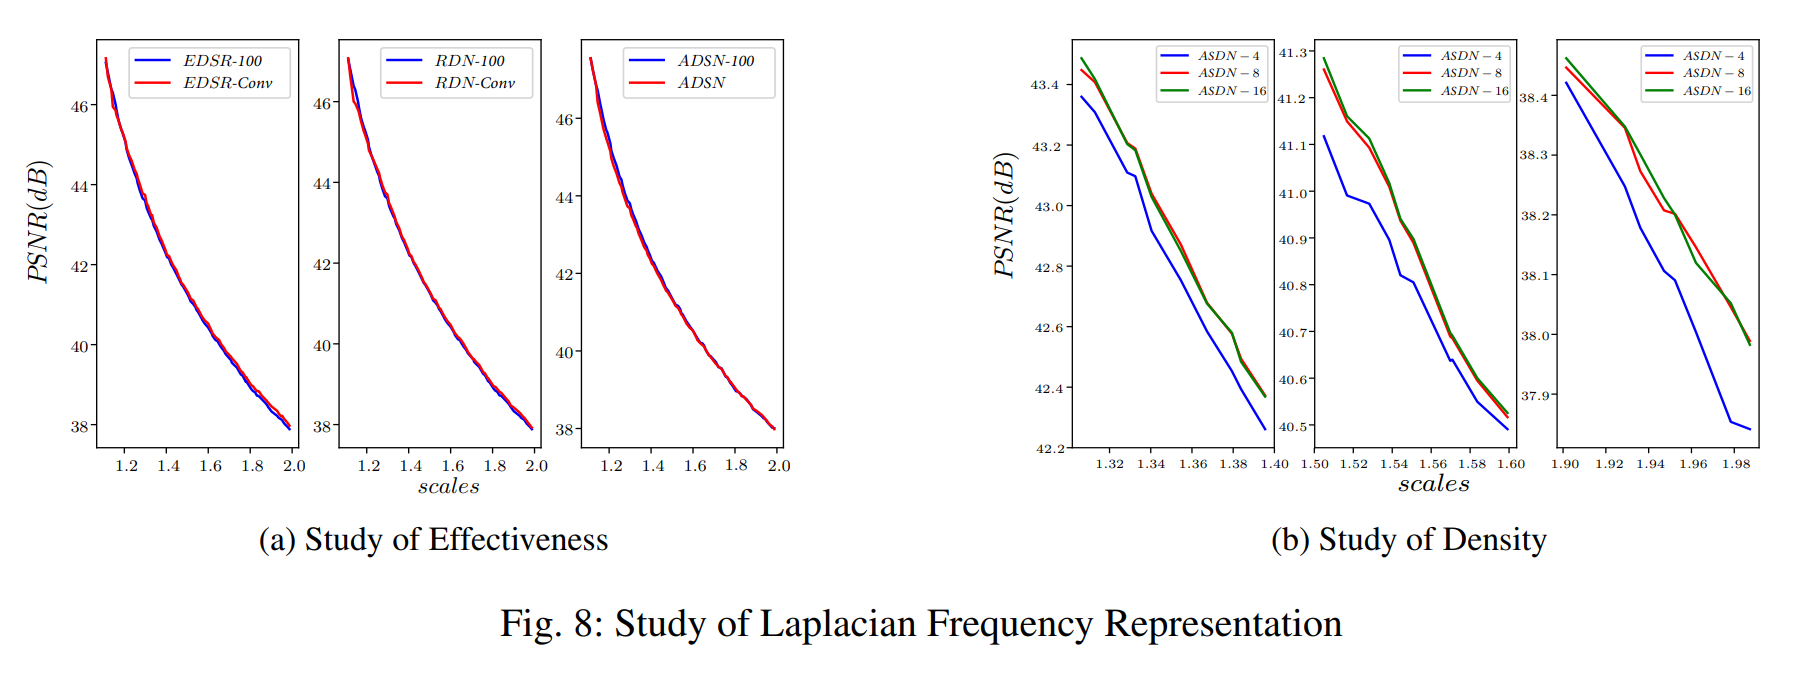
\includegraphics[width=0.9\textwidth, keepaspectratio]{asdn-study-lfr.png}
        \end{figure}
        \begin{itemize}
            \item ESDR-100, RDN-100, ASDN-100: upsampling networks trained and tested on 100 scales between (1,2] on Set5.
            \item ESDR-Conv, RDN-Conv, ADSN: networks trained as ASDN with 11 IRBs.
            \item ASDN-4,8,16: networks with 5,9,17 levels in the LFR with a scales range between (1,2]
            \item A denser LFR is better but saturate beyond 10 phases (11 levels).
        \end{itemize}

    }

    % Recursive redeployment
    \only<6>{
        \framesubtitle{Recursive deployment}
        \begin{itemize}
            \small
            \item Learning the mapping for any scale is too complex.
            \item For scales greater than the maximum in the scale range apply recursively the network.
            \item A large scale \textit{R} can be expressed as an integer \textit{N} power of decimal ratio \textit{r}:
            $$R = r^N \Rightarrow N= \log_r R$$
            \item Was found that using the greatest r at the beginning lead to better performance
            \item Since the range is fixed between (1,2] then $$\left\lceil N=\log_2 R \right\rceil$$ and therefore
            $$r_i = 
            \begin{cases}
                2 & \text{i } \le \text{N - 1} \\
                \frac{R}{2^{N-1}} & \text{i}=\text{N} \\
            \end{cases}
            $$
        \end{itemize}
    }
    \only<7>{
        \framesubtitle{Study of recursive deployment - Effectivness}
        \begin{figure}
            \centering
            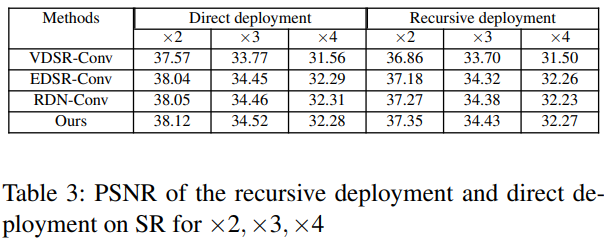
\includegraphics[width=0.6\textwidth, keepaspectratio]{asdn-study-rd.png}
        \end{figure}
        \begin{itemize}
            \item \textit{recursive deployment}: VDSR-Conv, EDSR-Conv, RDN-Conv, ASDN trained on 11 decimal scales in (1,2] and tested with HR images upscaled twice $$\sqrt2, \sqrt3, \sqrt4$$ in order to generate X2, X3, X4 HR images (therefore 2 recursions).
            \item \textit{direct deployment}: VDSR-Conv, EDSR-Conv, RDN-Conv, ASDN trained on images upsampled directly X2,X3,X4.
            \item \textbf{Recursive deployment} lead to worst performance but the difference goes down with the scale.
        \end{itemize}
    }

    \only<8>{
        \framesubtitle{Study of recursive deployment - Optimal N and r}
        \begin{figure}
            \centering
            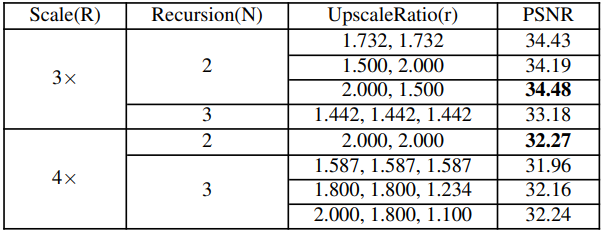
\includegraphics[width=0.6\textwidth, keepaspectratio]{asdn-study-n-rd.png}
        \end{figure}
        \begin{itemize}
            \item Different combination of N and r.
            \item Use the greatest r in the scales range at the beginning lead to better performance.
        \end{itemize}
    }

    \only<9-10>{
        \framesubtitle{Architecture}
        \begin{figure}
            \centering
            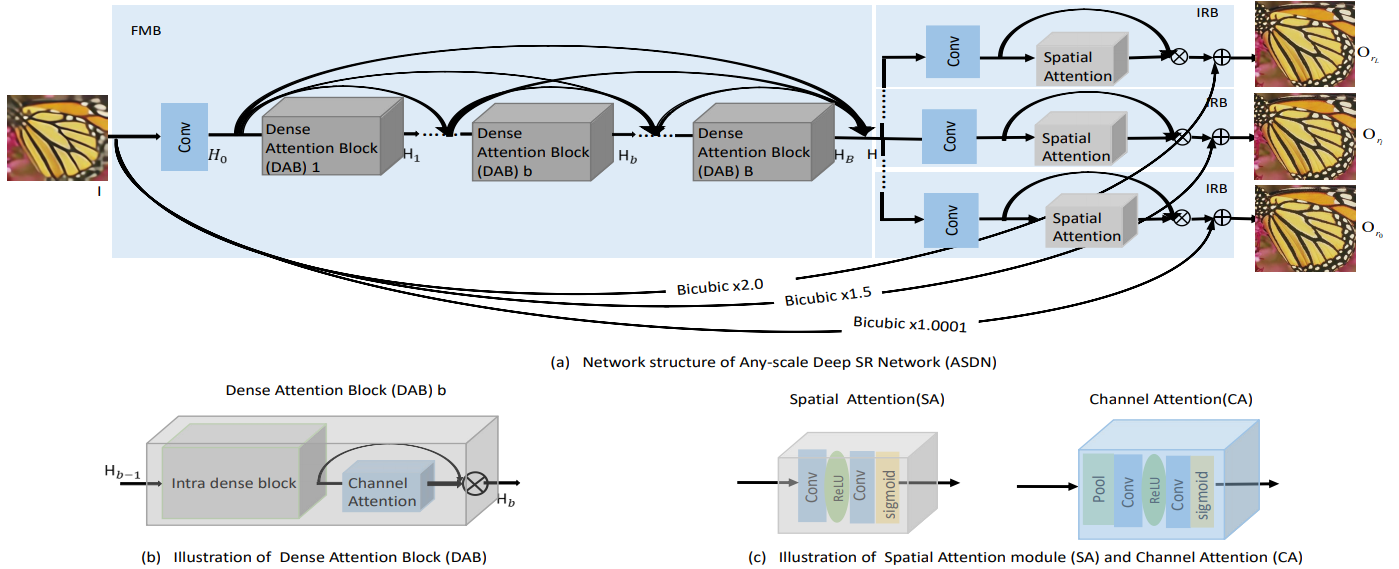
\includegraphics[height=0.4\textheight, keepaspectratio]{asdn-architecture.png}
        \end{figure}
    }
    \only<9>{
        \begin{itemize}
            \tiny
            \item Bi-dense connections (DAB with IDB) for learning efficiently features (since DenseNet, SRDenseNet and RDN doesn't allow previous features to be used into next blocks).
            \item IDB contains convolutions whose activations are processed with ReLu (without BN in order to maintain image details), densely connected convolutions and convolutions for compressing the input and the output (which is summed with the compressed input).
            \item CA from RCAN in order to focus on most important features.
            \item SA from CSFM in order to focus on particular and important textures at the reconstruction.
            \item Two IRBs are activated based on the scale used for training or testing and the the final image is reconstructed using the formula seen before. 
            \item Global skip connection for including low frequency information from the input and allow the network to learn high frequency information only.
        \end{itemize}
    }
    \only<10>{
        \begin{itemize}
            \item All convolutions have 64 filters and 3x3 kernel size with 0-padding and stride equals to 1 but the ones in IRB (1x1 kernel and 3 filters), CA (1x1 kernel which reduce-expand the channels), SA (1x1 kernel which expand-reduce the channels).
            \item Number of DABs: 16.
            \item Number of convolutions inside IDBs: 8.
        \end{itemize}
    }

    \only<11>{
        \framesubtitle{Training}
        \begin{itemize}
            \small
            \item Dataset used: DIV2K and Flicker
            \item At each update each IRB is randomly selected and combined after FMB
            \item The input LR images are bicubic interpolated from the training images with 11 decimal ratios r in evenly distributed in the range of \text{(1,2]}.
            \item In each training batch, 16 augmented RGB patches with the size 48x48 are extracted from LR images as the input, and the LR images are randomly selected from one scale training samples among the total 11 scales training data.
            \item In the training batch, a batch of 96x96 size patches is used as targets and the corresponding scale LR RGB patches to optimize the specific scale modules.
            \item Data augmentation: horizontal flip and 90-degree rotation.
            \item Use Adam ( default parameters ) with L1 loss and lr is halved at every 200000 minibatch updates for 1000000 total minibatch updates. 
        \end{itemize}
    }
    \only<12>{
        \framesubtitle{Testing}
        \begin{itemize}
            \item Dataset used: Set5, Set14, BSD100, Urban100 and Manga109.
            \item Testing images are first downscaled with the test scale s (randomly selected).
            \item If the scale s is not large than 2, the LR images with scale s are upsampled and forwarded into the ASDN with two enabled neighboring Laplacian pyramid levels of the scale s and HR image are predicted interpolating this two levels.
            \item If the scale s is large than 2, the testing is done recursively $$\left\lceil \log_2R \right\rceil$$ 
        \end{itemize}
    }
\end{frame}

\begin{frame}{FSDN - Fixed-Scale Deep Network}
    \begin{itemize}
        \item Fine-tune ASDN for a specific scale.
        \item Same structure of ASDN.
        \item A deconvolutional layer is inserted before IRB.
        \item Training: LR images downscaled by 2x,3x,4x,8x based on the specific scale and trained on the specific scale.
        \item Testing: LR images downscaled and forwarded into the network for returning the corresponding output.
    \end{itemize}
\end{frame}

\begin{frame}{ASDN : Results}
    \only<1>{
        \framesubtitle{Fixed-scale}
        \begin{columns}
            \begin{column}{0.5\textwidth}
                \begin{figure}
                    \centering
                    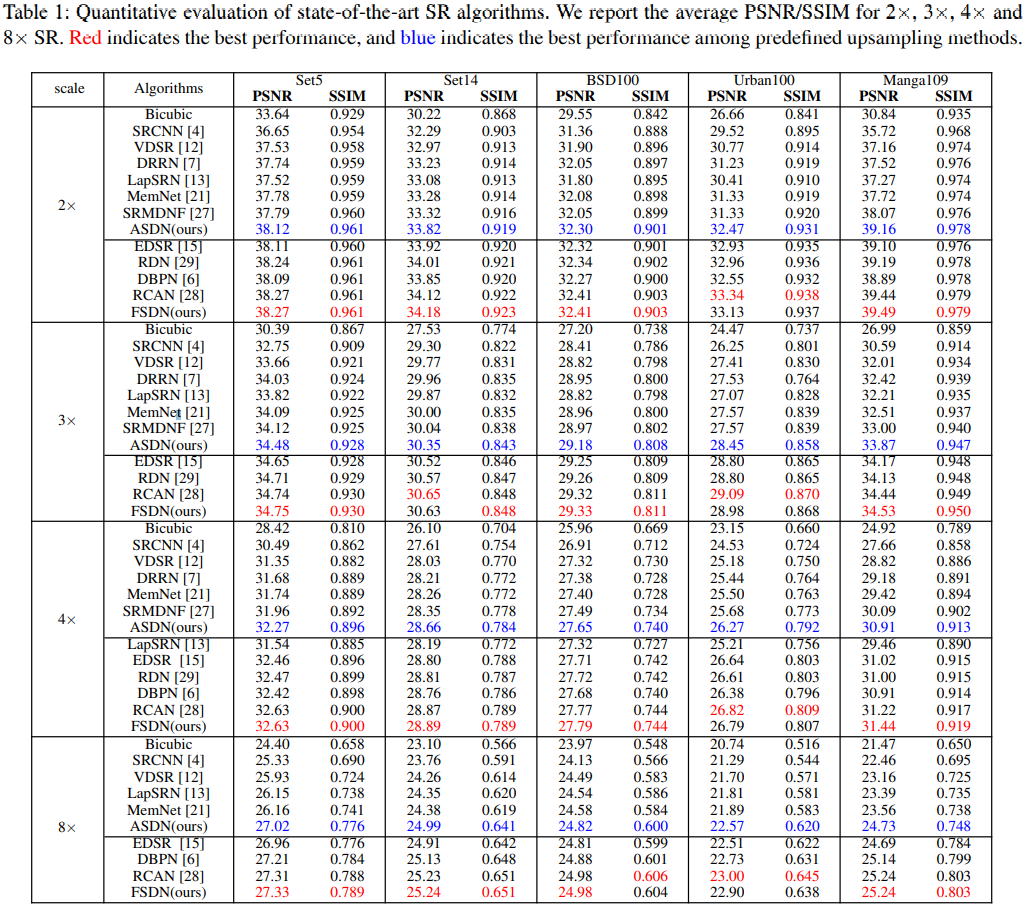
\includegraphics[width=\textwidth,height=200px]{asdn-table1.png}
                \end{figure}                    
            \end{column}
            \begin{column}{0.5\textwidth}
                \begin{itemize}
                    \tiny
                    \item Overall FSDN is better than SOTA networks up to now.
                    \item RCAN is sometimes better due to more channel attention layers which allow better reconstruction.
                    \item ASDN is better than other networks in all fixed scales although it is trained in the range (1,2].
                    \item Sometime ASDN performs worst than other networks because they are trained on specific scales with specific upsampled modules (transposed convolution) not usable with decimal ratios. The meta-upsampling module can be used only on scales used for training. Indeed FSDN performs better than ASDN due to the transposed convolution.
                \end{itemize}                    
            \end{column}
        \end{columns}
    }
    \only<2>{
        \framesubtitle{Any-scale}
        \begin{columns}[onlytextwidth]
            \begin{column}{0.5\textwidth}
                \begin{figure}
                    \centering
                    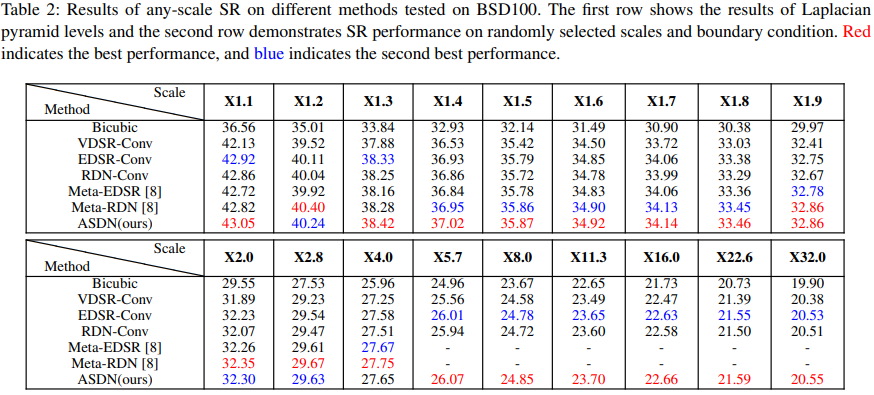
\includegraphics[width=\textwidth, keepaspectratio]{asdn-table2.png}
                \end{figure}
                \begin{figure}
                    \centering
                    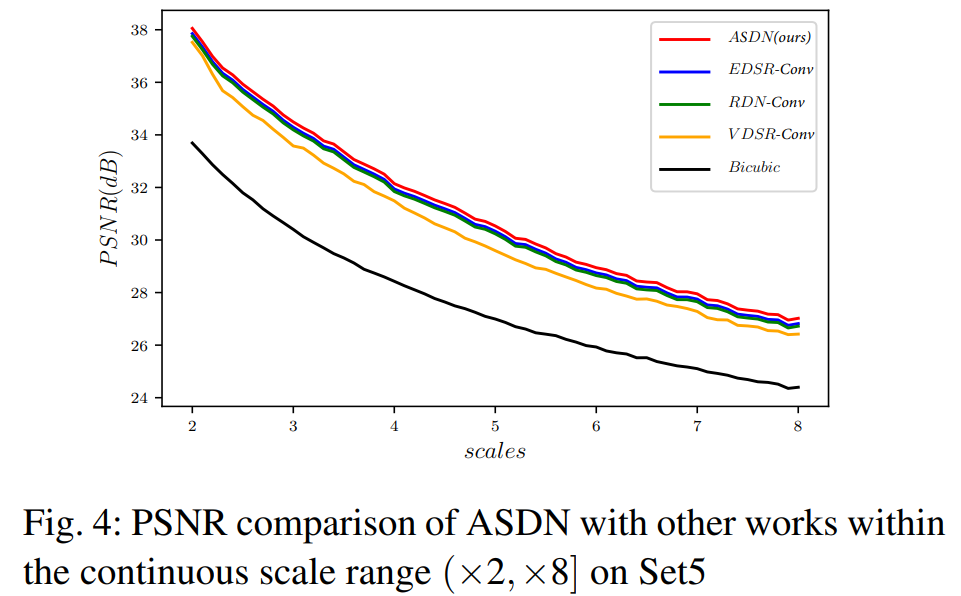
\includegraphics[width=\textwidth, keepaspectratio]{asdn-fig4.png}
                \end{figure}                    
            \end{column}
            \begin{column}{0.5\textwidth}
                \begin{center}
                    \begin{itemize}
                        \tiny
                        \item VDSR-Conv, EDSR-Conv,RDN-Conv are networks trained as ADSN
                        \item Meta-EDSR, Meta-RDN are networks with a meta-upscaling module trained with scales range between [1,4] with stride 0.1
                        \item ASDN and networks trained as ASDN perform better on continuos (random) scales between 1 and 8.
                    \end{itemize}                        
                \end{center}
            \end{column}
        \end{columns}
    }
    \only<3>{
        \framesubtitle{Qualitative comparison}
        \begin{figure}
            \centering
            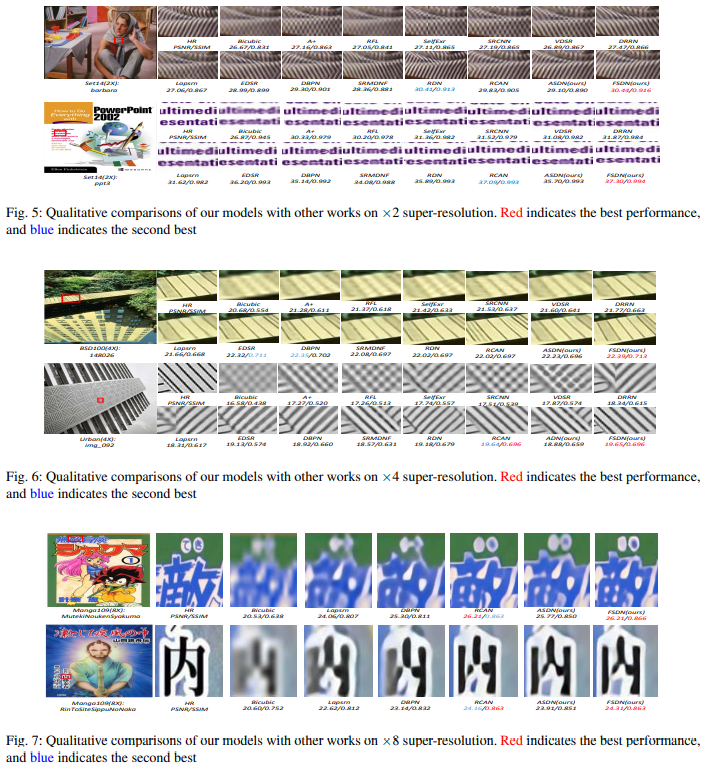
\includegraphics[height=0.88\textheight, keepaspectratio]{asdn-qulitative-results.png}
        \end{figure}
    }
\end{frame}

\begin{frame}{ASDN}{Model analysis}
    \begin{figure}
        \centering
        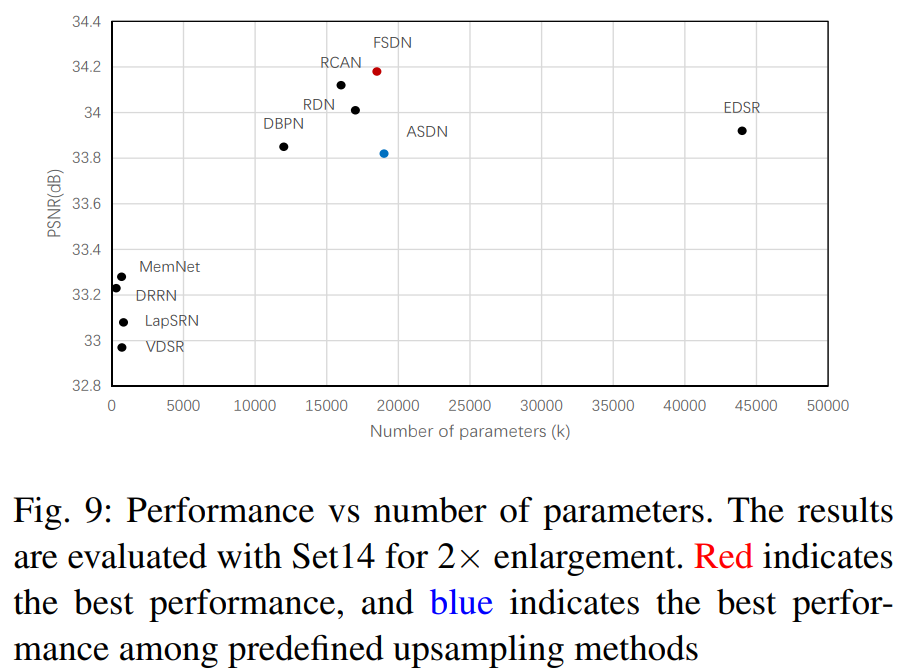
\includegraphics[height=0.5\textheight,keepaspectratio]{asdn-psnr-n_params.png}
        \vspace*{100px}
        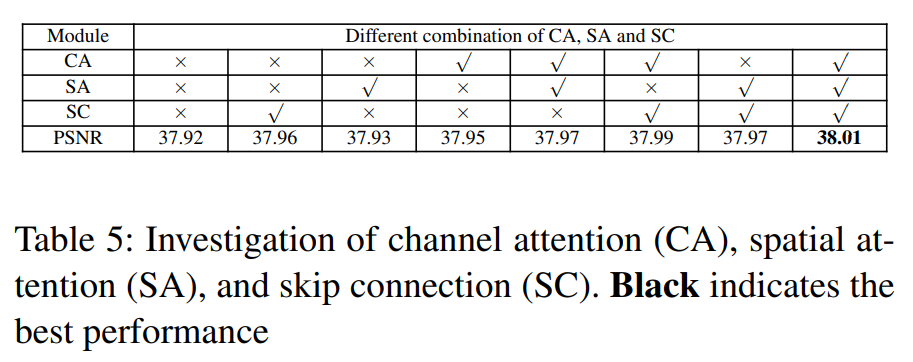
\includegraphics[height=0.5\textheight,keepaspectratio]{asdn-ablation-study.png}
    \end{figure}
\end{frame}



% EXTRA 
\begin{frame}{Extra}
    % Set subtitles
    \only<1-2>{
        \section{Laplacian Pyramid}\label<1>{section:LaplacianPyramid}
        \framesubtitle{Laplacian pyramid\cite{laplacianpyramid}}
    }
    \only<3-4>{
        \section{DBDN}\label<3>{section:DBDN}
        \framesubtitle{DBDN: Deep Bi-Dense Networks for image SR \cite{DBDN}}
    }
    \only<5-6>{
        \section{MetaSR}\label<5>{section:MetaSR}
        \framesubtitle{Meta-SR: A Maginfication-Arbitrary Network for SR \cite{MetaSR}}
    }
    \only<7-8>{
        \section{RCAN}\label<7>{section:RCAN}
        \framesubtitle{RCAN: Image SR using very deep Residual Channel Attention Networks \cite{RCAN}}
    }
    \only<9-10>{
        \section{CSFM}\label<9>{section:CSFM}
        \framesubtitle{CSFM: Channel-wise and Spatial Feature Modulation Network for Single Image SR \cite{CSFM}}
    }
    \only<11-12>{
        \section{LapSRN and MS-LapSRN}\label<11>{section:LapSRN}
        \framesubtitle{LapSR and MSLapSR: Fast and accuracte Image SR with Deep Laplacian Pyramid Networks \cite{LapSRN} \cite{MSLapSRN}}
    }

    % Set frames content
    \only<1>{
        \begin{itemize}
            \small
            \item Generate images with high frequency information only subtracting filtered images with itself non filtered: similar to apply a laplacian operator on the image.
            \item Remove correlation between pixels.
            \item Those images can be used for reconstructing the original image.
            \item Hand crafted kernel for filtering the image in order to cutoff low frequency (low-pass filtering) information:
            \begin{itemize}
                \tiny
                \item Separable
                \item Symmetric
                \item Normalized: $$a + 2b + 2c = 1$$
                \item Equal contribution: $$a + 2c = 2b$$
                \item Kernel = 
            \end{itemize}
        \end{itemize}
        \begin{columns}
            \begin{column}{0.3\textwidth}
                \begin{figure}
                    \centering
                    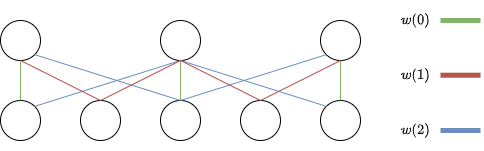
\includegraphics[width=100px,keepaspectratio]{laplacianpyramidexample.png}
                    \caption{Equal contribution.}
                \end{figure}        
            \end{column}
            \begin{column}{0.6\textwidth}
                \begin{itemize}
                    \tiny
                    \item All nodes in the lower level must have the same contribution to nodes in the upper level. 
                    \item The central node contributes with a + 2c
                    \item The middle ones contribute with 2b
                    \item The outer ones with a + c
                    \item So a+2c=2b
                \end{itemize}
            \end{column}
        \end{columns}
    }
    \only<2>{
        \begin{figure}
            \centering
            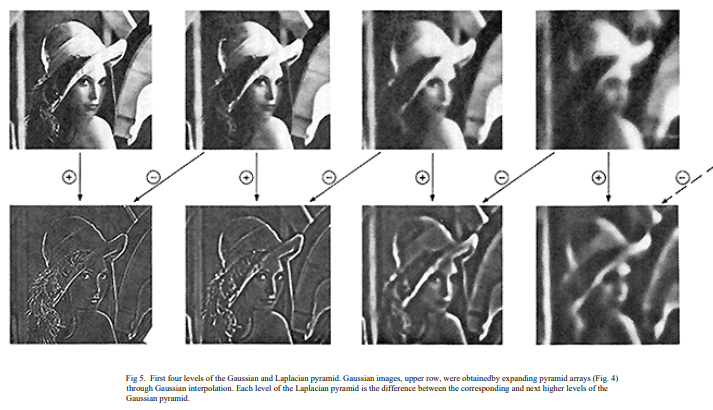
\includegraphics[width=0.9\textwidth]{laplacian-pyramid example.png}
        \end{figure}
    }
    
    \only<3>{
        \begin{itemize}
            \item Deeper network lead to better performance
            \item The deeper the network is the more likely the vanishing/exploding gradient is present.
            \item Use skip connections (with sum). 
            \item Reuse features thanks to dense connection (with concatenation) for improving final results.
            \item The flow is limited from one block to another: features are not really reused.
        \end{itemize}
        \begin{figure}
            \centering
            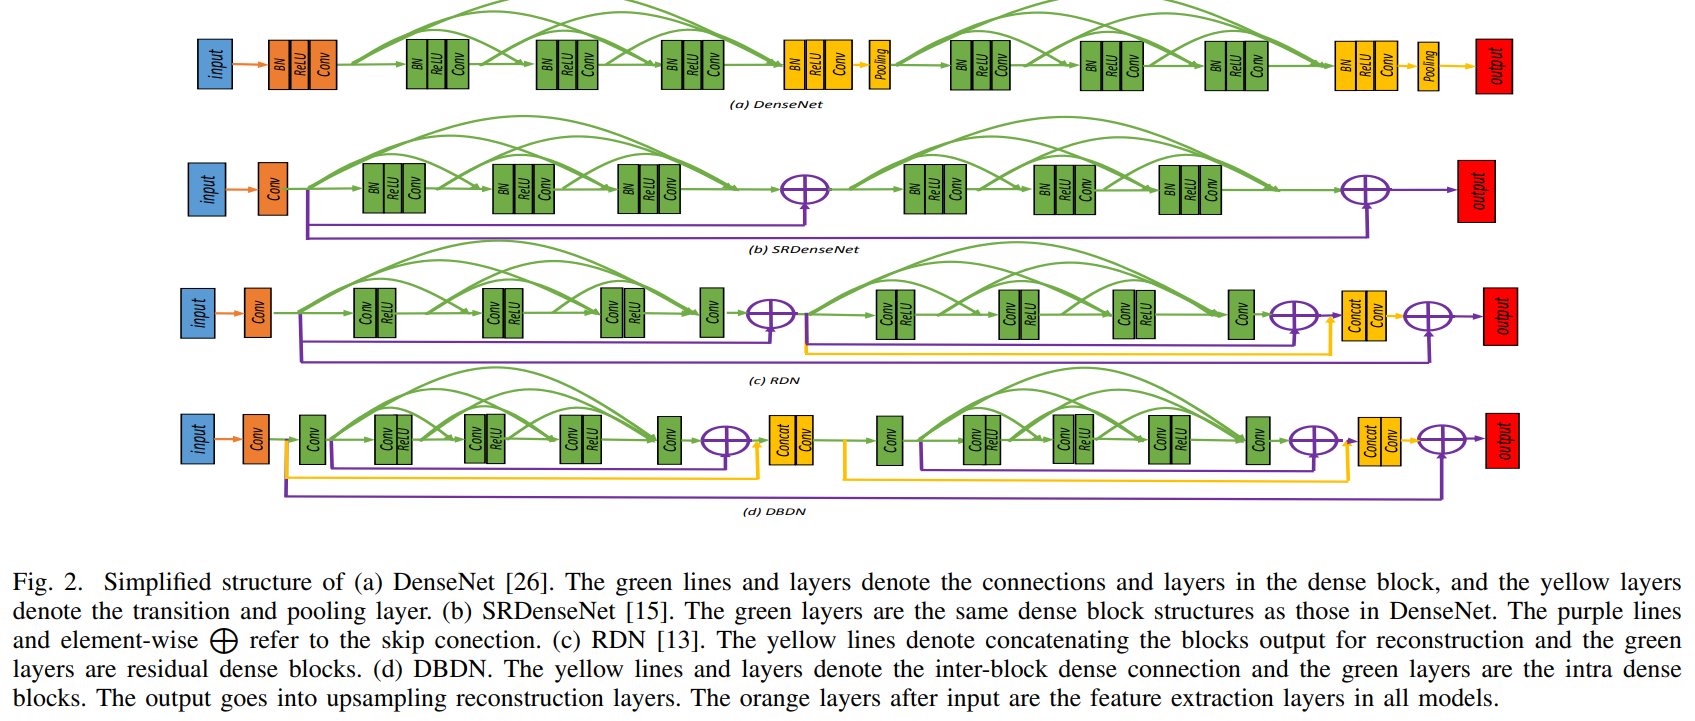
\includegraphics[height=0.4\textheight, keepaspectratio]{bidense-comparison.png}
        \end{figure}
    }
    \only<4>{
        \begin{figure}
            \centering
            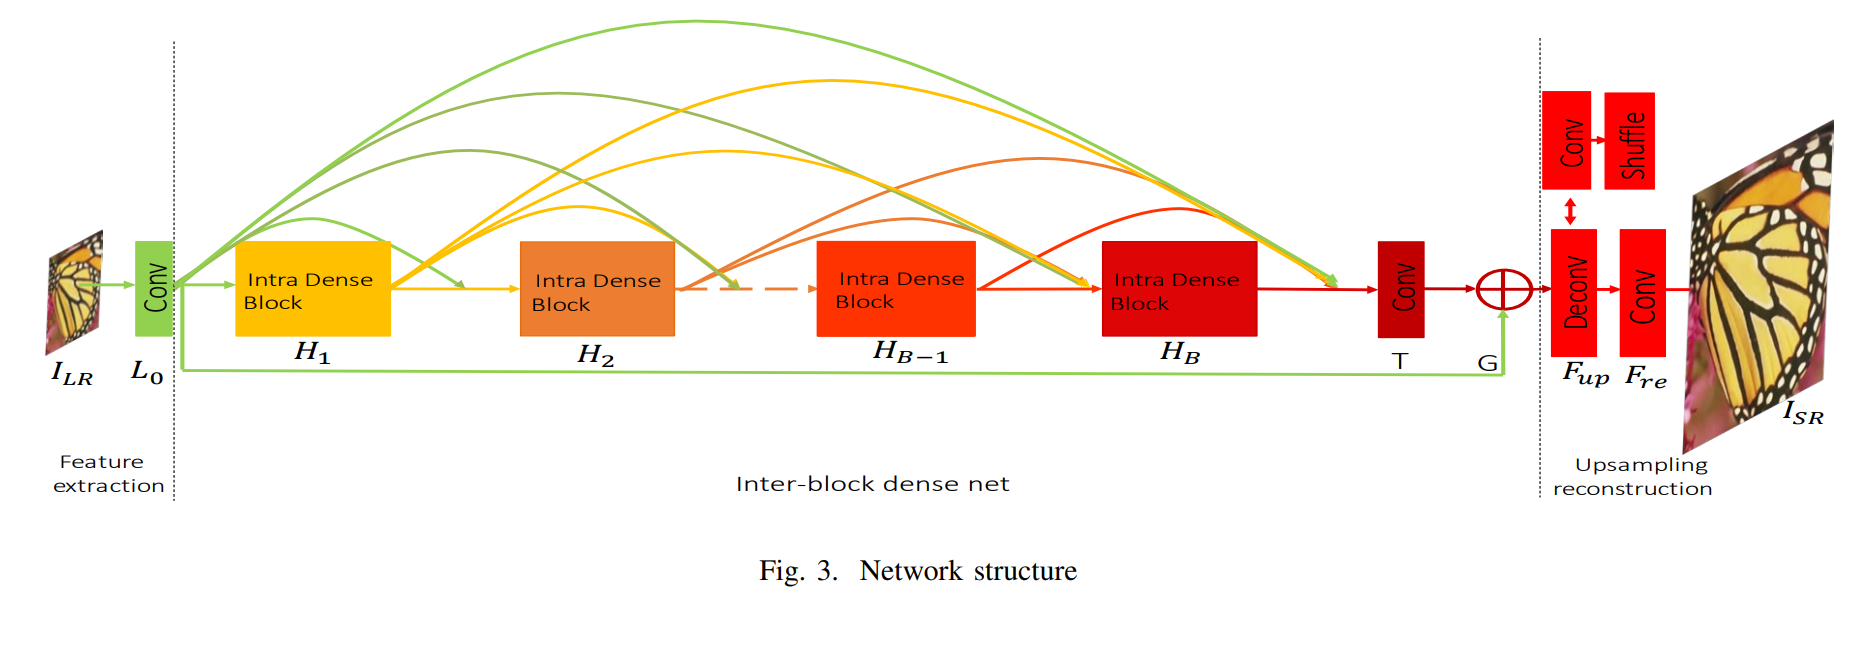
\includegraphics[height=0.37\textheight,keepaspectratio]{bidense-model.png}
        \end{figure}
        \begin{figure}
            \centering
            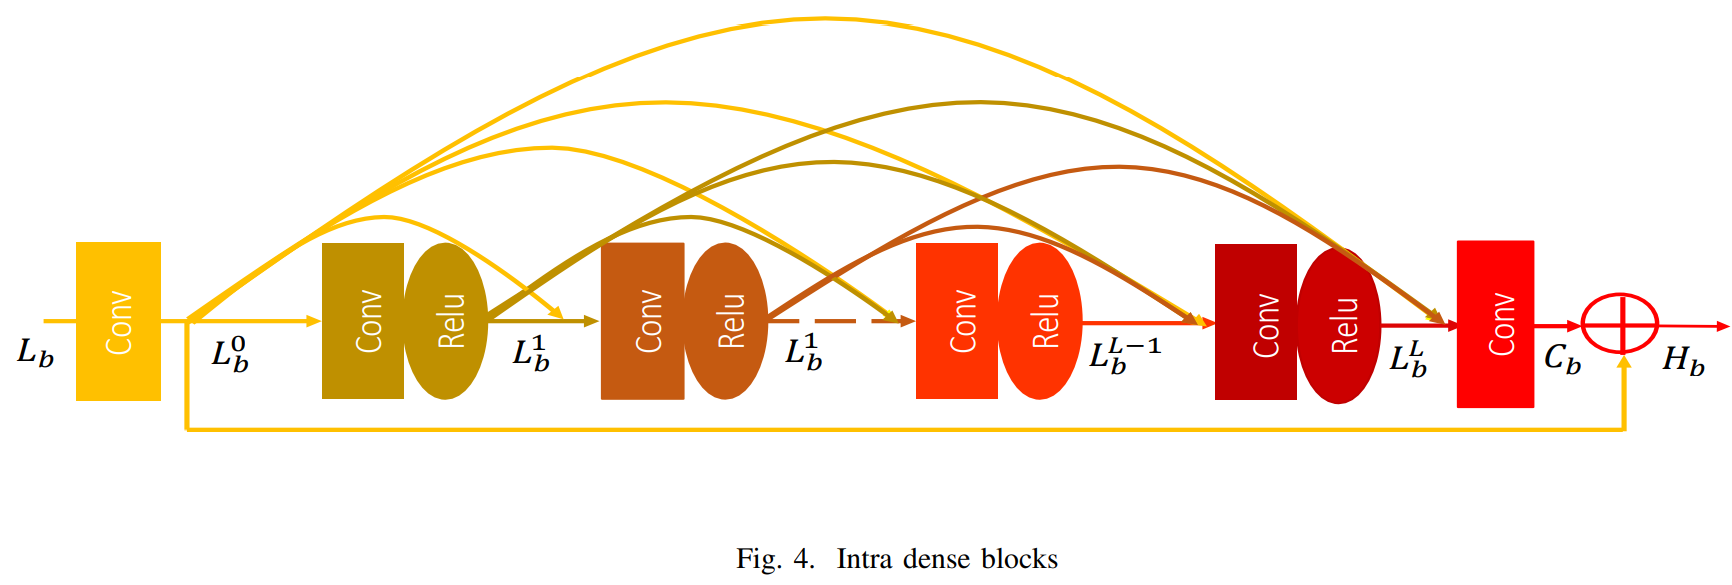
\includegraphics[height=0.37\textheight,keepaspectratio]{bidense-intra-dense-block.png}
        \end{figure}
    }

    \only<5>{
        \begin{itemize}
            \item SR for a specific integer scale as independent task: memory-wise and time-wise costly ( since you have to train and maintain data and models ) .
            \item The same hold with decimal scale.
            \item Meta-SR exploit \textbf{meta-learning} creating \textbf{meta-upscale} module which allow to learn to generate weights based on the input scale and therefore use one network for all possible \textit{trained} scales.
        \end{itemize}
            \begin{figure}
                \centering
                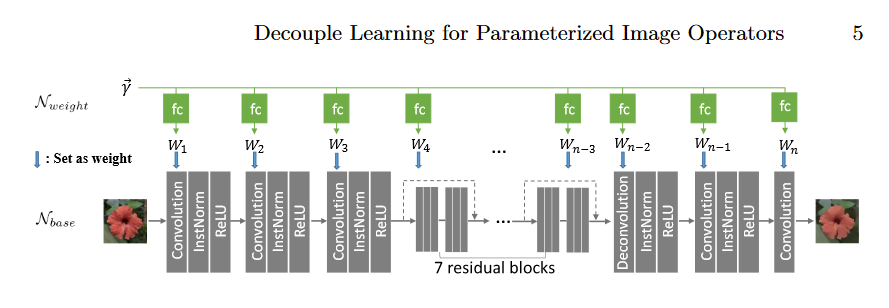
\includegraphics[scale=0.4]{paramsimageoperatormodel.png}
                \caption{Meta-learning on Parametrized Image Operators \cite{ParametrizedImageOperator}}
            \end{figure}
    }
    \only<6>{
        \begin{figure}
            \centering
            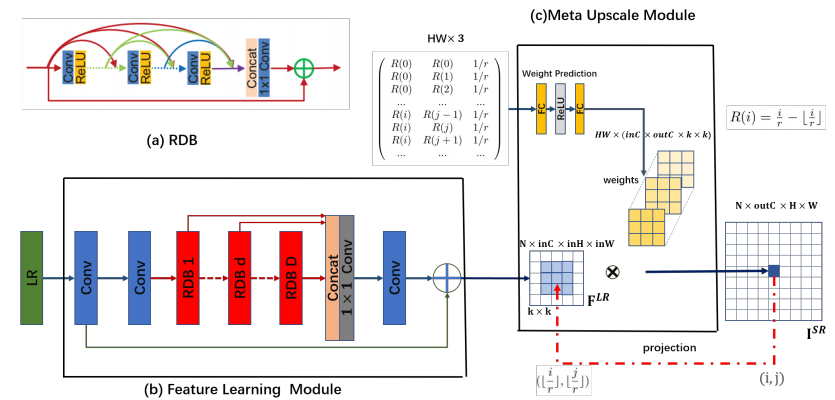
\includegraphics[height=0.5\textheight, keepaspectratio]{metasr-model.png}
        \end{figure}

        \textbf{Meta Upscale Module}:
        \begin{itemize}
            \tiny
            \item \textit{location projector}: project pixel in HR to LR image
            \item \textit{weight prediction}: predicts the weights of the kernels using a fully connected network (2 layers with 256 hidden units and ReLU as activation)
            The input is vector of offset (proper choice) and scales (in order to differentiate different scales during training therefore learn different weight for different scales).
            \item \textit{feature mapping}: reconstruct the image as the matrix product between the features extracted and the weights computed.
        \end{itemize}
    }

    
    \only<7>{
        \begin{itemize}
            \item Deep networks are very effective for CV tasks
            \item This lead to vanishing/exploding gradients, hence skip connections are used in order to avoid these.
            \item The LR image contains low-frequency information
            \item The processed features inside the network contain high-frequency information.
            \item Increase the performance focusing the learning of high-frequency information using \textbf{attention}.
        \end{itemize}
    }
    \only<8>{
        \begin{figure}
            \begin{subfigure}{0.45\textwidth}
                \centering
                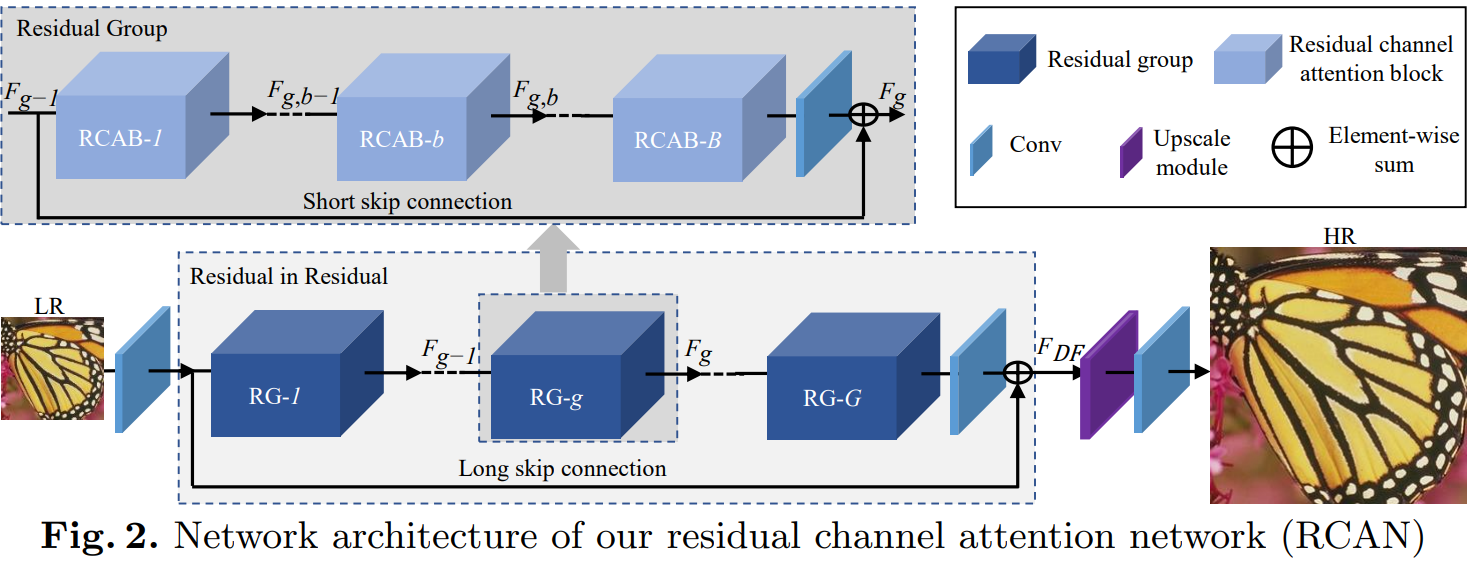
\includegraphics[width=\textwidth, keepaspectratio]{rcan-model.png}                    
            \end{subfigure}
            \begin{subfigure}{0.45\textwidth}
                \begin{subfigure}{\textwidth}
                    \centering
                    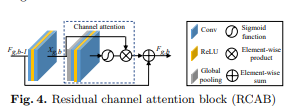
\includegraphics[width=\textwidth, keepaspectratio]{rcan-rcab.png}
                \end{subfigure}    
                \begin{subfigure}{\textwidth}
                    \centering
                    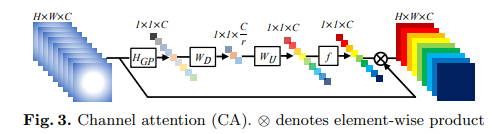
\includegraphics[width=\textwidth, keepaspectratio]{rcan-channel-attention-module.png}
                \end{subfigure}                
            \end{subfigure}
        \end{figure}
        \begin{itemize}
            \item \textbf{Residual-in-Residual}: allow to build a deeper network as well as allow to flow low-frequency information from shallow levels to deeper levels easing the training. 
            \item \textbf{Channel-wise attention}: Increase the performance of the network focusing on most important channel-wise features.
        \end{itemize}
    }

    \only<9>{
        \begin{itemize}
            \item Use deeper network for higher performance.
            \item Use residual and dense connections for avoiding exploding/vanishing gradient.
            \item Use residual and dense connection for features reusing and flowing most important information in the network.
            \item Exploit attention channel-wise and spatial-wise for learning high-frequency information and information on most important region.
        \end{itemize}
    }
    \only<10>{
        \begin{columns}
            \begin{column}{0.5\textwidth}
                \begin{figure}
                    \begin{subfigure}{\textwidth}                
                        \centering
                        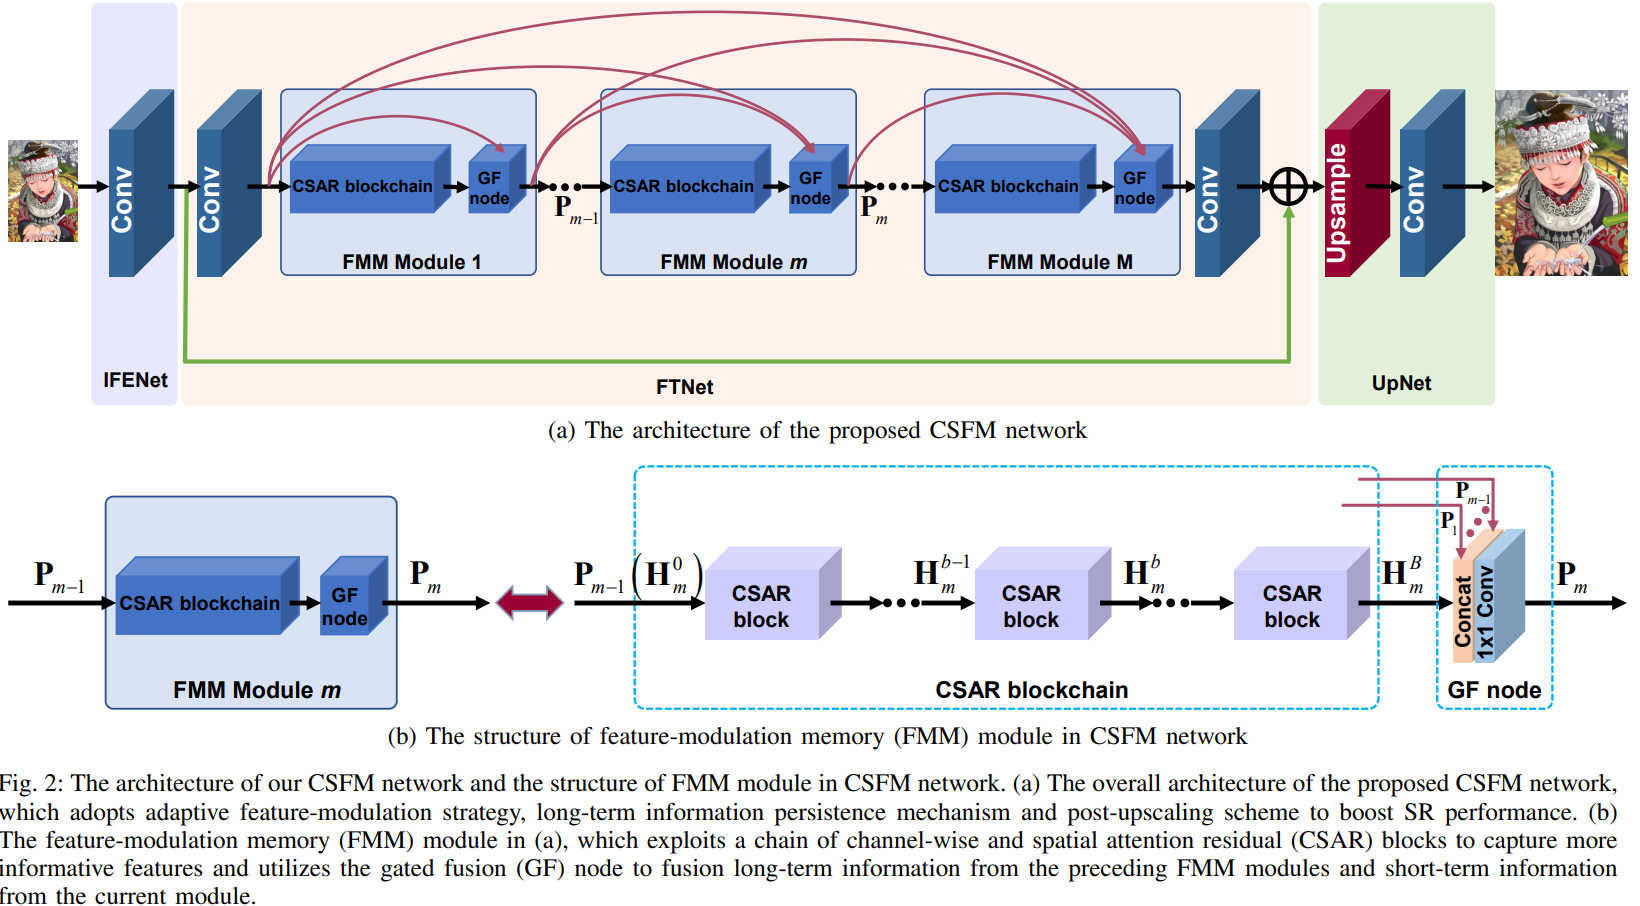
\includegraphics[width=\textwidth, keepaspectratio]{csfm-model.png}
                    \end{subfigure}
                    \begin{subfigure}{\textwidth}                
                        \centering
                        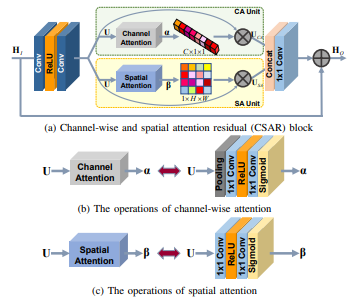
\includegraphics[height=0.45\textheight, keepaspectratio]{csfm-csar-module.png}
                    \end{subfigure}            
                \end{figure}                        
            \end{column}
            \begin{column}{0.5\paperwidth}
                \begin{itemize}
                    \small
                    \item Use FMMs for exploiting channel and spatial information as well as create a memory using the GF node.
                    \item The CSAR blockchain allow to capture most important features information and flow these into the FMM module.
                    \item The GF node concatenate the current CSAR blockchain output and all previous FMM outputs for preserving long-term information and also create new features for SR image reconstruction.
                \end{itemize}
            \end{column}
        \end{columns}
    }

    \only<11>{
        \textbf{LapSRN}        
        \begin{itemize}
            \tiny
                \item L2 loss fail to capture one-to-many mapping between LR and HR patches: use \textbf{Charbonnier loss}:
                $
                L_S = \frac{1}{N} \sum_{i=1}^{N}\sum_{l=1}^{L} \rho \times \left( \left( y_l^{(i)}-x_l^{(i)} \right) - r_l^{(i)} \right)
                $
                where \textit{S} is the target upsampling factor, $L=\log_2 S$,  $\rho = \sqrt{x^2+\epsilon^2}$ (Charbonnier penalty function, differentiable variant of L1 norm).

                \item Apply the upsampling operator at the end (previous papers apply it at the beginning increasing inference and training time): \textbf{transposed convolution} or \textbf{subpixel convolution}.
                \item Single upsampling step lead to worst performance: \textbf{reconstruct progressively} the SR image using a laplacian pyramid framework \cite{laplacianpyramid}.
        \end{itemize}
        
        \textbf{MS-LapSRN}
        \begin{itemize}
            \tiny
            \item \textbf{Parameter sharing} within (reuse of the same recursive blok) pyramid levels and across pyramid levels (reuse of the same feature extractor).
            \item Use of \textbf{skip connections} for avoiding vanishing/exploding gradients
            \item \textbf{Multi-scale training} (in the previous work they trained different network for each scale: 2x,4x,8x)
        \end{itemize}
    }   
    \only<12>{
        \begin{columns}[T]
            \begin{column}{0.5\textwidth}
                \begin{figure}
                    \begin{subfigure}{\textwidth}
                        \centering
                        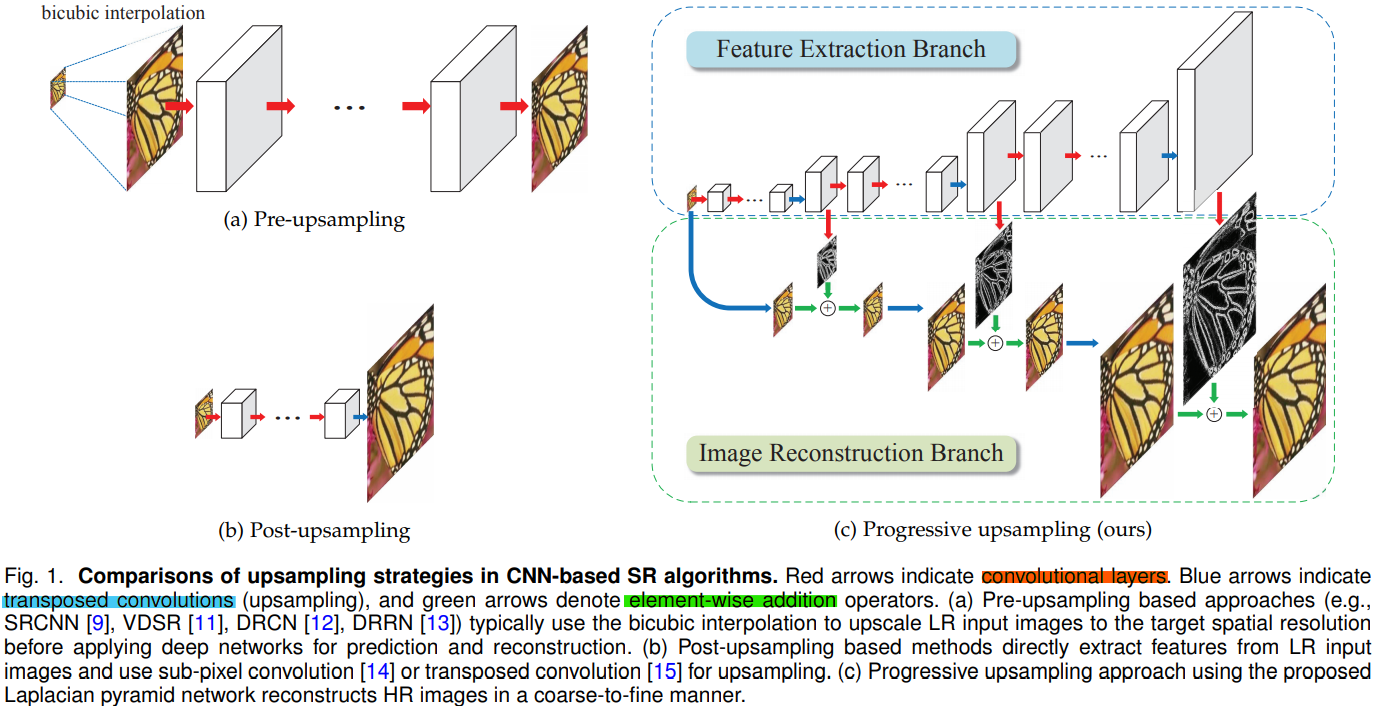
\includegraphics[width=\textwidth, keepaspectratio]{lapsr-old-model.png}                            
                    \end{subfigure}
                    \begin{subfigure}{\textwidth}
                        \centering
                        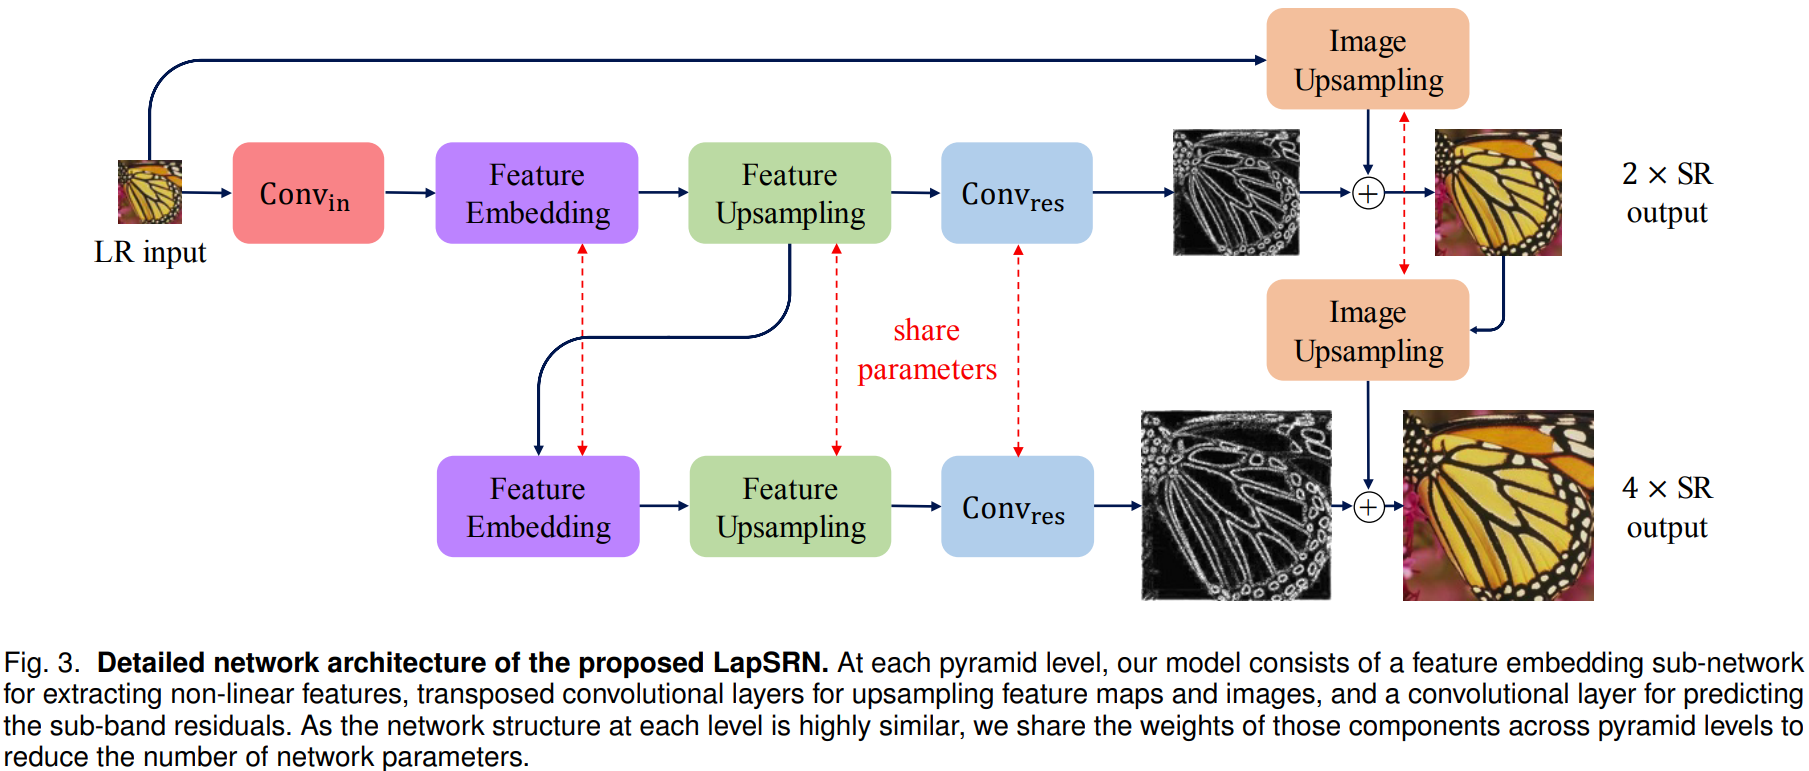
\includegraphics[width=\textwidth, keepaspectratio]{lapsr-new-model.png}                            
                    \end{subfigure}
                \end{figure}                        
            \end{column}
            \begin{column}{0.5\textwidth}
                \begin{figure}
                    \begin{subfigure}{\textwidth}
                        \adjustimage{height=0.29\textheight, keepaspectratio, cfbox=LightPurple 2pt}{lapsr-recursive-block-differences.png}
                    \end{subfigure}
                    \begin{subfigure}{\textwidth}
                        \adjustimage{height=0.29\textheight, keepaspectratio,cfbox=LightPurple 2pt}{lapsr-recursive-block.png}
                    \end{subfigure}
                \end{figure}                        
            \end{column}
        \end{columns}
    }   

\end{frame}

\bibliographystyle{ieeetr}
\bibliography{../bibliography}

\end{document}